\documentclass[10pt,twocolumn,letterpaper]{article}

\usepackage{cvpr}
\usepackage{times}
\usepackage{epsfig}
\usepackage{graphicx}
\usepackage{amsmath}
\usepackage{amssymb}

% Include other packages here, before hyperref.

% If you comment hyperref and then uncomment it, you should delete
% egpaper.aux before re-running latex.  (Or just hit 'q' on the first latex
% run, let it finish, and you should be clear).
\usepackage[breaklinks=true,bookmarks=false]{hyperref}

\cvprfinalcopy % *** Uncomment this line for the final submission

\def\cvprPaperID{****} % *** Enter the CVPR Paper ID here
\def\httilde{\mbox{\tt\raisebox{-.5ex}{\symbol{126}}}}

% Pages are numbered in submission mode, and unnumbered in camera-ready
%\ifcvprfinal\pagestyle{empty}\fi
\setcounter{page}{1}
\begin{document}

%%%%%%%%% TITLE
\title{Image Generation Using Generative Adversarial Nets}

\author{Ang Li\\
Boston University\\
{\tt\small anglli@bu.edu}
% For a paper whose authors are all at the same institution,
% omit the following lines up until the closing ``}''.
% Additional authors and addresses can be added with ``\and'',
% just like the second author.
% To save space, use either the email address or home page, not both
\and
Lan Luo\\
Boston University\\
{\tt\small julerrie@bu.edu}
\and
Tianyu Gu\\
Boston University\\
{\tt\small mygty21@bu.edu}
}

\maketitle
%\thispagestyle{empty}

%%%%%%%%% ABSTRACT
\begin{abstract}
In this project, we implemented Principal Component Analysis(PCA) and Generative Adversarial Nets(GANs) for image generation problem. Taking the MNIST and CelebA datasets as training data, the model generates new images that mimic the images in dataset alike. This paper introduces working principles of GANs and discusses the differences between different implementations and the foundings during experiments.
\end{abstract}

%%%%%%%%% BODY TEXT
\section{Introduction}

Image generation has been a prevalent topic for the research in machine learning area in recent years. The goal of image generation is to produce images which has a similar appearance to the images in the training data set. To a broader view, the task of generating images requires a promising ability to modeling or representing the high-dimensional probability distribution, as images are good examples of high-dimensional data that subject to a certain distribution. Knowing the distribution of the images, we can generate the samples following such distribution hence producing the images that may look alike. Generative models are used to accomplish this task on representing the probability distribution of the real data, like Gaussian Mixture Model. In such a way, we are able to let the model learn from the extensive data in a certain domain, hence in a way "understand" the data. Such model could be used in different applications such as denoising, superresolution and so on.\\

The probability distribution of the images is unknown, which we denote as $P_{data}$. One of the methods to represent that $P_{data}$ is to explicitly define a data distribution, denoted as $P_{model}$, to model the $P_{data}$, which is usually designed as a parametric model and then train the $P_{model}$ by methods such as Maximum Likelihood(ML) estimation over the training set. In this manner, $P_{model}$ is imposed to be a good estimation of $P_{data}$. Sometimes it is not necessary for generative modeling to have an explicit model defined. Instead of obtaining the data distribution as the target, one could have only the data generated from the $P_{model}$ without explicitly define the $P_{model}$ by some assumption, like a black box. GANs[1] is an example of this.\\

This project is focused on the study and practical performance evaluation of GANs. One remarkable point of GANs is the method of training. One of the traditional approaches of training is based on minimizing the MSE of the generated samples and the ground truth. But GANs applies a different approach of training in a adversarial way. In some applications such as image super-resolution, the adversarial training produces a more clearer and sharper results than the MSE method.[2]

%------------------------------------------------------------------------
\section{Related Works}

During our study of image generation problem and on generative models, a common method is to obtain the $p_{model}$ by maximizing the likelihood of $\sum_{i=1}^{n}p_{model}(x_i)$ over $n$ training samples. Such method is equivalent to train the parameters for $p_{model}$ that maximized summation of log-likelihood instead of the product of likelihood in order to simplify the computation. We can consider this  maximize likelihood (ML) estimation as minimizing the Kullback-Leibler(KL) divergence of the $p_{model}$ and $p_{data}$:
\begin{align}
\theta &= argminD_KL(p_{data}||p_{model})\nonumber \\
&= argmin\sum_{i=1}^{n}p_{data}(x_i)log\frac{p_{data}(x_i)}{p_{model}(x_i;\theta)}
\end{align}

There are several works that are based on the above idea or similar.In our study of the related topics, different generative models based on the idea of maximum likelihood have critical performances. Two related works are introduced in this paper, each manifest a typical way of modelling and maximum likelihood estimation, which illustrates the maximum likelihood approach in tractable and intractable form. As the idea of GANs differs from the related works, the details of the related works are not discussed here.

%-------------------------------------------------------------------------
\subsection{PicelCNN}

PixelCNN, and PixelRNN[3][4], model the conditional distribution for each pixel given the existence of the other pixels in the image, usually the pixels on the up or left direction. The maximum likelihood could then be performed on the product of conditional distributions of all the pixels, similar to Naive Bayes[5], but this method does not consider each pixel is independent, so the conditional distribution is applied. This approach has a simple and clear design, which allows a straightforward ML estimation. But the running time of this approach is not desirable as for each image it is required to model the conditional distribution of all the pixels in the image, which is an O(n) time complexity that could possibly make the algorithm not efficient.


%-------------------------------------------------------------------------
\subsection{Variational Autoencoder(VAE)}

Variational Autoencoder(VAE)[6] is another approach for image generation. The model matches the training samples into a latent vector z and then generate the samples using the latent vector z. This model is not parametrically designed with a tractable form of the $p_{model}$, rather, the model is intractable for directly maximum likelihood estimation. Rather than maximum likelihood estimation of $p_{model}$, VAE maximizes the lower bound of the log likelihood of $p_{model}$ as an approximation way. This method provides a novel way of training, but in practice the generation result is usually blurred. This illustrated the solution when the model is intractable for ML estimation. But the GANs is different from the above two examples.


%-------------------------------------------------------------------------
\section{Generative Adversarial Nets}
Generative Adversarial Nets (GANs) is a novel framework that is first introduced by Lan Goodfellow \textit{et al.} in 2014. As the name suggests, GANs is consist of two adversarial models, the generator denoted as G and the adversarial discriminator model as D.\\

\textbf{Generative net}: 
The generator is a parametric model that aims to estimate the probabilistic distribution of the training data pdata by constructing a mapping function between a simple prior distribution $p(z)$  and the $p_{data}$. In other words, through the training process, the generator is capable of minimizing the difference between the $p(x|\theta,z)$ and $p_{data}$.\\ 

\textbf{Discriminative net}:
Similarly, the discriminator is a parametric model that aims to differentiate whether a input image $x$ is drawn from the dataset. Specifically, for the input data image x and generated image $g(z)$, the D is trained to simultaneously maximize the $D(x)$ and minimize the  $D(G(z))$. Therefore, It can be considered as a binary classifier of which the output could represent the possibility that x belongs to the dataset.   


%-------------------------------------------------------------------------
\subsection{Training as gameplay}

In GANs, the training process can be considered as a gameplay in which the generator G is keep competing with the discriminator during the training process. As discussed above, the discriminator is trying to distinguish the real data samples from the fraudulent images that generated from the G. on the other hand, by maximizing the possibility of the D being correct, or in other words, by trying to "fool" D, the G could generate more authentic image and thus, learning the pdata. Therefore, during the training process, It is expected that, by updating their own parameters,  the G would generate more authentic image as the performance of D increases. Ideally, the Generator will be able to generate data samples that are similar enough to the real data samples. At that time, Discriminator can not determine where the input data comes from, which means D(x) will close to $\frac{1}{2}$ for all data samples. The whole training process is illustrated by Figure 1 as below. 
\begin{figure}[h]
\begin{center}
   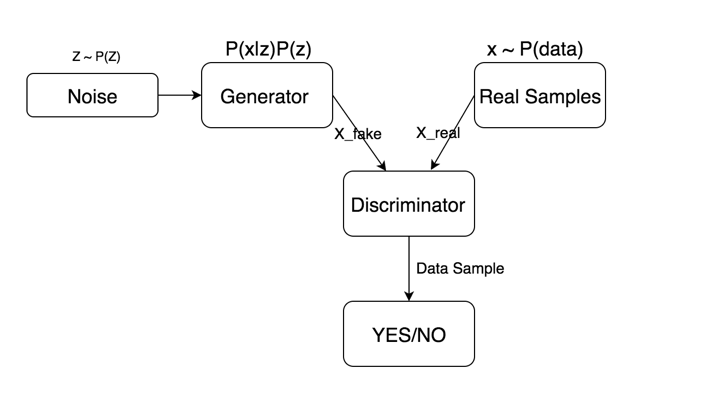
\includegraphics[width=\linewidth]{img/frame.png}
\end{center}
   \caption{A simple diagram that shows the training process of GANs. Here, half of the discriminator input, denoted as $x$, are randomly selected from the datasets. While the other half are generated by the generator based on the prior distribution $z$.	}
\label{fig:long}
\label{fig:onecol}
\end{figure}


%-------------------------------------------------------------------------
\subsection{The Cost functions and its properties  }
\textbf{General forms}: As discussed above, the cost function of G and D should be adversarial with each other in some way. More specifically, the cost function of the generator and discriminator should have the following forms:
\begin{align}
L_G = J^{(G)}(\theta^{(D)},\theta^{(G)})\\
L_D = J^{(D)}(\theta^{(D)},\theta^{(G)})
\end{align}
Where, $\theta^{(D)}$ and $\theta^{(G)}$ are the trainable parameters for model G and D respectively. Note that, G and D will try to minimize their own cost function with only the control of their own parameters, Moreover, by assuming the game as a zero-sum game, which means setting $L_G+ L_D =  0$, minimizing one cost function will direct result in maximizing the other.\\

\textbf{Nash Equilibrium}:
Mathematically, the solution towards the above gameplay would be a tuple ((D),(G)) that achieves the Nash Equilibrium. That is to say, the solution ((D),(G))should satisfies the requirement that, for any infinitesimal perturbation on the (D) or  (G), the corresponding cost function of G and D could not be further minimized. In practice, researches have been using the stochastic gradient descent simultaneously for G and D to find the equilibrium point ((D),(G)). However, there is no guarantee that such optimization algorithm will finally converge and the theoretical analysis of the conditions on convergence is still an open research problem.\\
   	
\textbf{The Discriminative Net's cost function}:
So far, most of the proposed GANs adapt the same cost function:
\begin{align}
J^{D(\theta^{D},\theta^G)}&= -\frac{1}{2}E_{x~p_{data}}log(D(x)) -\frac{1}{2}E_z(1 - D(G(z))\\
		       &= -\frac{1}{n}\sum_{i=1}^{n}[y_{data}log(D(x)) + (1 -y_{generated})log(1 -D(G(z))   
\end{align}
This is nothing but the cross-entropy cost function for the sigmoid output of D. In practice, all the training labels for real data samples ydata and generated sample ygenerated are set to be 1 or 0 respectively. Therefore, by minimizing the equation (*), the D would maximize the D(x) and minimize the D(G(z)) simultaneously.\\

The advantage of this particular cost function is that, for a fixed generator?s output, the D is always trying to estimate the ratio between the probabilistic distribution of the data samples pdata and the generated samples, pmodel, and correspondingly assign the labels to each group. This can be proved by the following equations:
For a fixed (G), the optimal(D) for equation <*> would be:
 		(D)* = argmin(theta) equations ~\\
		
Therefore, we can conclude that, in each step of the training, with enough capacity, the D will re-estimate the $\frac{p_{data}}{p_{model}}$ for every pixel in the image, and assign the labels for the images correspondingly.  This will not only improve the performance of D but also serves as a guide for the generator's training process.\\

\textbf{The generative net's cost function}:
If we keep the training process as a zero-sum gameplay, then the generator's cost function will be:
<equation 2> 
For a optimal (D)* , the above equation could be rewritten as:
Here the KL is...Therefore, the minimal value of the above function is achieved as $p_{model}$ = $p_{data}$. Hence, the performance of the generator will increase as   

%------------------------------------------------------------------------
\section{Implementation}
With the recent intensive study in neural networks, several approaches of image generation are modeled into the neural network, GANs is also implemented by different forms of the neural networks. 
Neural network[7] is system which models different functions using the connected artificial neurons with certain activation functions. The topic of neural networks is not explained in detail as is beyond the major scope of this paper. Convolutional Neural Network(CNN)[8] is based on neural networks but having a different architecture which is more robust than ordinary neural networks. Normally the CNN takes an image as input and convolve with several small sized kernels which are called filters. Then the result of the convolution is downsampled. This process repeats regarding the number of layers of the CNN is designed. Finally the output is reshaped as a vector and is fed to fully connected neurons, called fully connected layer, and the final result is produced.
In GANs, the G and D are implemented separately, usually with different kinds of neural networks. In this project, the two GANs are implemented. One is using the ordinary artificial neural networks as both G and D. The other one is using Convolutional Neural Networks(CNN) as both G and D, which follows the architecture of DCGAN[9], an extended work of GANs based on CNN.
\subsection{PCA}
\begin{figure}[h]
\begin{center}
   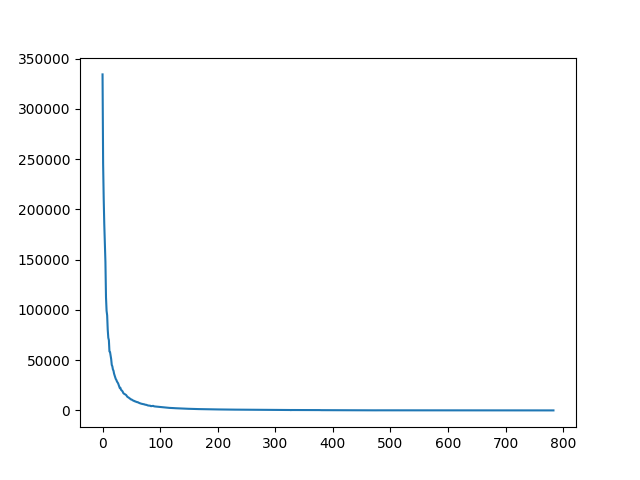
\includegraphics[width=0.8\linewidth]{img/pcaeigplot.png}
\end{center}
   \caption{The plot of eigenvalues of the covariance matrix for PCA. We choose latent vector to be 100 dimension for conserving the information of the data.}
\label{fig:long}
\label{fig:onecol}
\end{figure}
To compare against the GANs, PCA is applied as a baseline for image generation. The idea using PCA to generate image is to reconstruct images from latent vectors in the subspace spanned by the principal components trained from the image dataset. Hence the major features of the images should be reconstructed by this mean. The PCA subspace is 100 dimensional and the latent vector is a 100 dimensional vector drawn from the uniform distribution.
\subsection{GAN(NN)}
In the artificial neural network implementation of GANs, both G and D are implemented as a 2-layer neural network which has 128 nodes in the hidden layer. The neural network in G takes the 100-dimensional latent vector as input and the output layer maps the dimension of the image that we want to generate. The neural network in D takes the image as input and output in a single node output layer as D(x). The networks are trained with stochastic gradient descent. In each iteration, the real images and the generated images from G are intputted to D with the same batch size.
\subsection{DCGAN}
The 4-layer CNN is implemented for both D and G, with 5x5 filters for the convolutional layer. With a consistent setting, the input layer of G is also 100 nodes. The architecture of D is same as an ordinary CNN as mentioned above, the fully connected layer has one node as the final output. The architecture of G is a CNN in a reversed architecture of D. It takes a 100 dimensional vector as input and pass to a fully connected layer and then reshape to a 2D matrix and pass to the convolutional layer and upsampling, which finally yields a 2D matrix having the same size of the image, which is the target output image.

\section{Experiments}
\subsection{Datasets}
\textbf{MNIST}: The MNIST database is a handwritten digits database. It contains 60000 samples for training set and 10000 samples for testing set, for which each sample is $28\times28$ pixels.\\
 
\textbf{CelebA}: The CelebA dataset contains over 200 thousands RGB face images in $108\times108$ resolution. The face images are subject to large diversities such as pose variation and backgrounds.
\subsection{Results}
The MNIST dataset is used for training all the three models: PCA, GAN(NN) and DCGAN. The CelebA dataset is used for training DCGAN.\\

\begin{figure}[h]
\begin{center}
   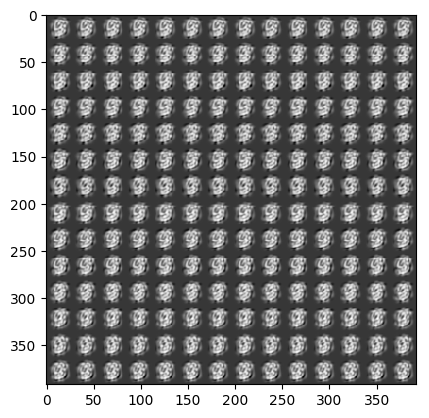
\includegraphics[width=0.6\linewidth]{img/pcaresult.png}
\end{center}
   \caption{PCA results for MNIST}
\label{fig:long}
\label{fig:onecol}
\begin{center}
   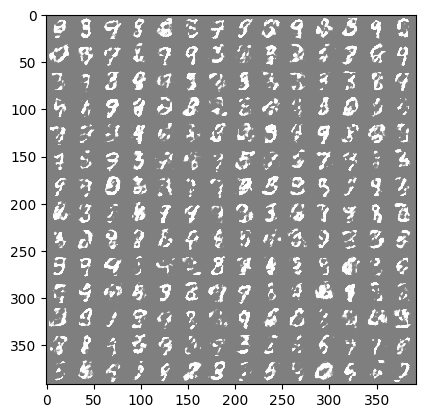
\includegraphics[width=0.6\linewidth]{img/gannn.png}
\end{center}
   \caption{GANs implemented with 2-layer neural networks results for MNIST}
\label{fig:long}
\label{fig:onecol}
\begin{center}
   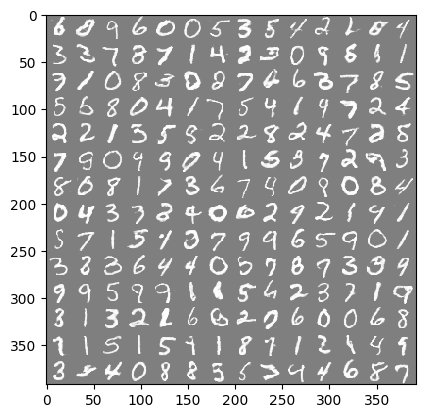
\includegraphics[width=0.6\linewidth]{img/dcgan.png}
\end{center}
   \caption{DCGAN results for MNIST}
\label{fig:long}
\label{fig:onecol}
\end{figure}
As can be seen from the results, in terms of the performance of different implementations, the DCGAN results is almost perfect on MNIST dataset, which also outperforms the other two implementations. From the PCA results we observed that the major features of the handwritten digits (white random strokes in the center and black background) are reconstructed, while the generated images are not even similar to any handwritten digits. This result also manifests the difficulty of general image generation problem as the images could subject to a broader distribution and it is hard to obtain the feature of a single digit rather than a general feature. The NN implementation of GANs has satisfactory results as most images look similar to the handwritten digits, although not clear enough.\\
\begin{figure}[h]
\begin{center}
   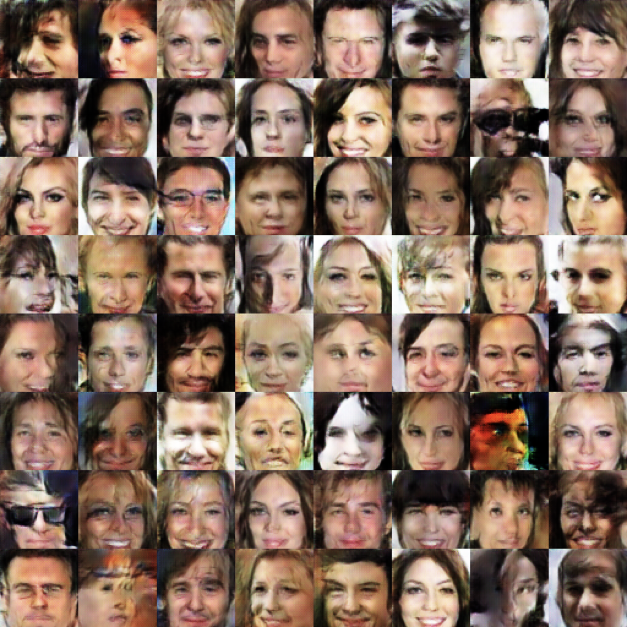
\includegraphics[width=0.6\linewidth]{img/celeb.png}
\end{center}
   \caption{DCGAN result for CelebA dataset}
\label{fig:long}
\label{fig:onecol}
\begin{center}
   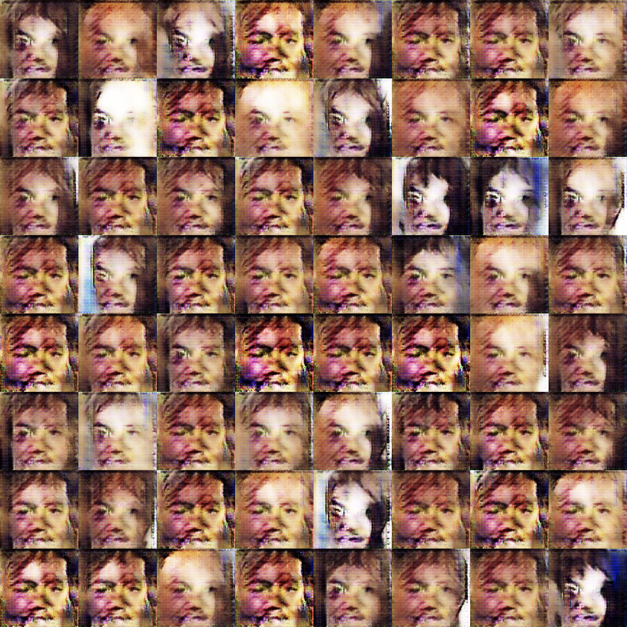
\includegraphics[width=0.6\linewidth]{img/celebfail.png}
\end{center}
   \caption{DCGAN result when unstableness observed, the quality of the outputs are severely worse}
\label{fig:long}
\label{fig:onecol}
\end{figure}

For CelebA dataset, the DCGAN result is better than expectation. The training time on an ordinary laptop is longer than we expected, and we saved the image generation result in the half way instead of running all the iterations, which could take several continuous days. Some of the images generated successfully mimic the feature of a human face and one can hard to tell the difference between those samples and real images and the other sample, although having a tilted face shape, also reconstructed some features of a human face, such as eyes and mouth.\\

During the experiment on CelebA dataset, we also found the unstableness of training the GANs as shown in Figure 7. While having a satisfactory result at a certain epoch, the next epoch suddenly exposes a drop in the performance, and the training loss increase sharply. We did not know the reason why this happened, but must be a limitation of the current implementation of the DCGAN.\\

\begin{figure}[h]
\begin{center}
   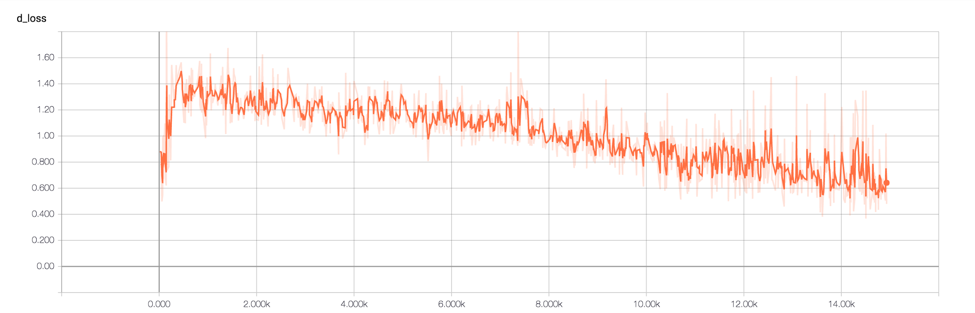
\includegraphics[width=\linewidth]{img/dloss.png}
\end{center}
   \caption{Loss of D with respect to number of iterations}
\label{fig:long}
\label{fig:onecol}
\begin{center}
   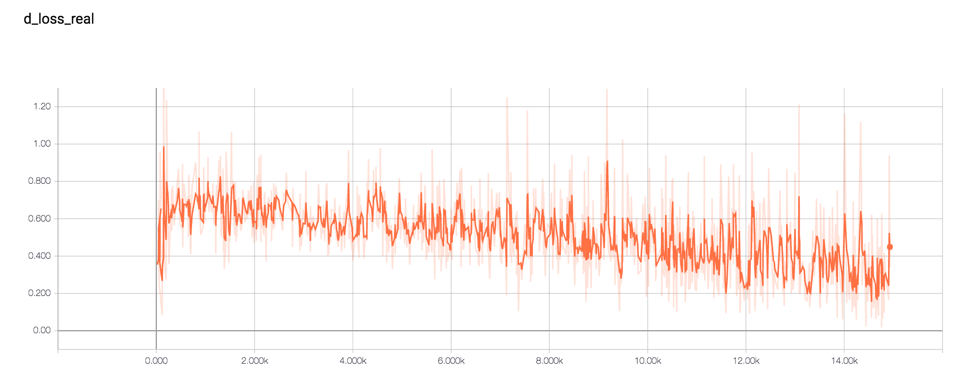
\includegraphics[width=\linewidth]{img/dlossreal.png}
\end{center}
   \caption{Loss of D for real images ($D(x^i)$) with respect to number of iterations}
\label{fig:long}
\label{fig:onecol}
\begin{center}
   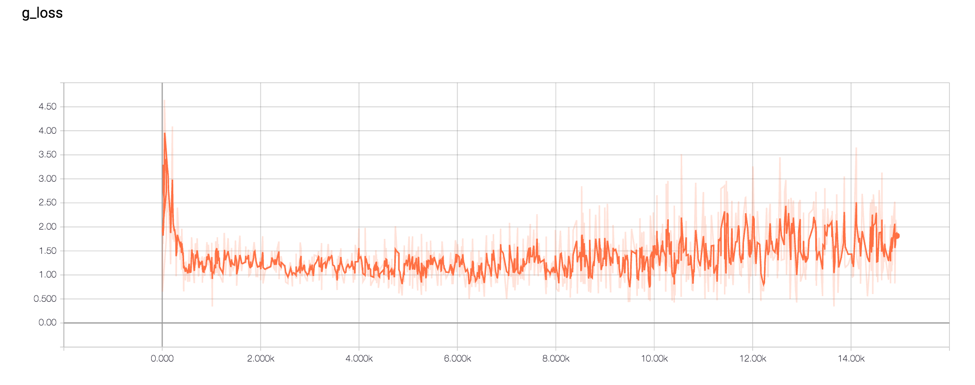
\includegraphics[width=\linewidth]{img/gloss.png}
\end{center}
   \caption{Loss of G with respect to number of iterations}
\label{fig:long}
\label{fig:onecol}
\end{figure}

From the loss plotted from we can see the loss of both G and D fluctuates and never converge smoothly like the ordinary gradient descent, as an outcome of the adversarial between the G and D. But in general, the loss of D(Figure 8) is decreasing over the number of iterations. The loss of D for real images(Figure 9) is also decreasing, meaning the D is increasing its ability to classify real images out of the whole batch while the loss of G(Figure 10) does not increase to a comparable extent with D, indicating the G is not losing the game for a more "powerful" D.\\

\section{Conclusion}
In this project, we showed the robustness of GANs as a generative model for image generation and also practiced the adversarial training method of GANs. Also, we found the training loss is hard to converge, not like the other modes training with gradient descent. Both loss for G and D keep fluctuating through the whole training process. Nash Equilibrium is hard to achieve, which is illustrated in the original GANs paper, and this limitation of GANs obviously arose during our experiments that sometimes the training loss increases sharply and the outputs become poor as mentioned above. This is also one of the future works that we think worth taking effort into, and there are already some publications on studying the instability of training a GANs model[10]. If some state of the art approaches could stabilize the training of the GANs, this generative model could be more robust on more broader tasks. Another question arisen from this project is how to quantify the evaluation of the image generation result. This is also our concern from day one. The solution for this problem that we think could be a mechanism of classifiers to providing a score for the generated results, which could serve as a benchmark for image generation problem.
{\small
\bibliographystyle{ieee}
\bibliography{egbib}
}

\end{document}
